\subsection{Analyse von Schaltkreis b)}\ref{kap:Spule}
\begin{figure}[h]
	\centering
	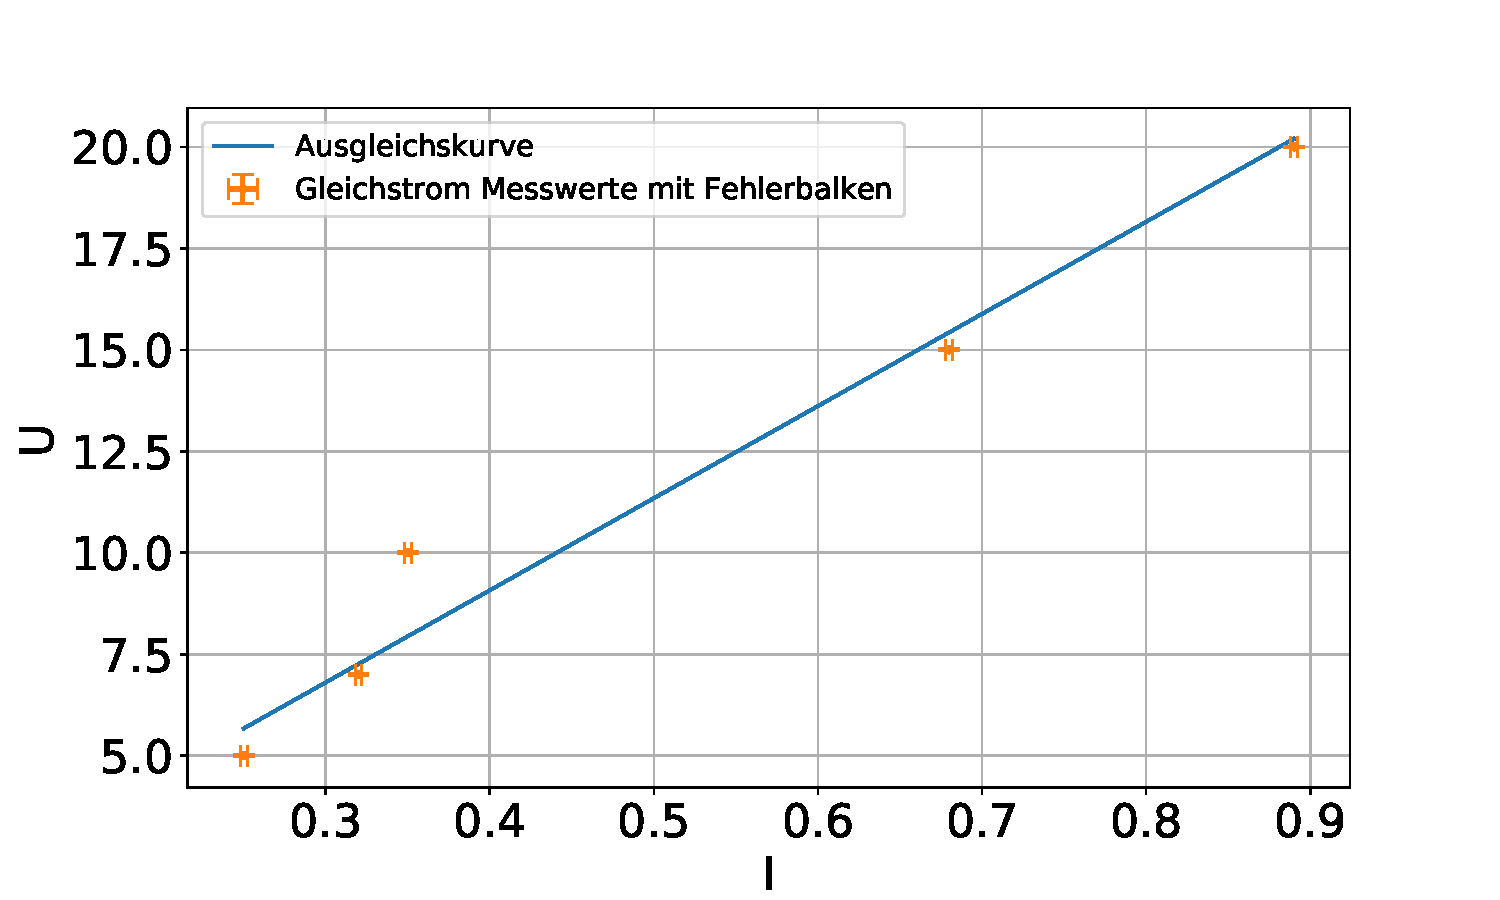
\includegraphics[width=0.9\textwidth]{res/UgegenI_GL.pdf}
	\caption{Die Spannung $U_{eff.}$ gegen den Strom $I_{eff.}$ für Gleichstrom.}
	\label{fig:UgegenIgl}
\end{figure}
\begin{figure}[h]
	\centering
	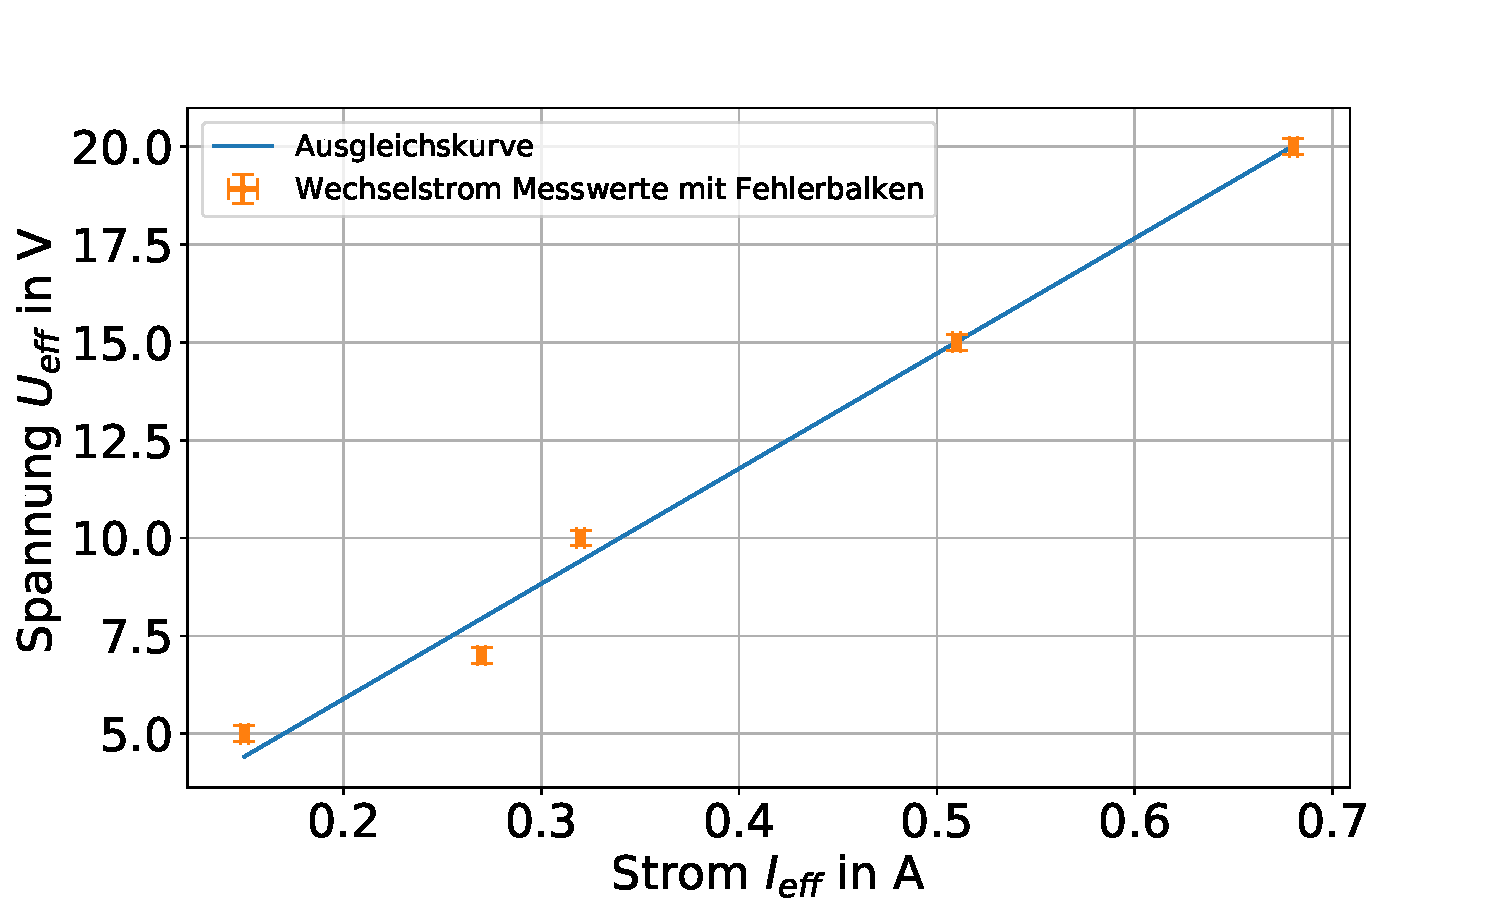
\includegraphics[width=0.9\linewidth]{res/UgegenI_W.pdf}
	\caption{Die Spannung $U_{eff.}$ gegen den Strom $I_{eff.}$ für Wechselstrom.}
	\label{fig:UgegenIw}
\end{figure}
\begin{figure}[h]
	\centering
	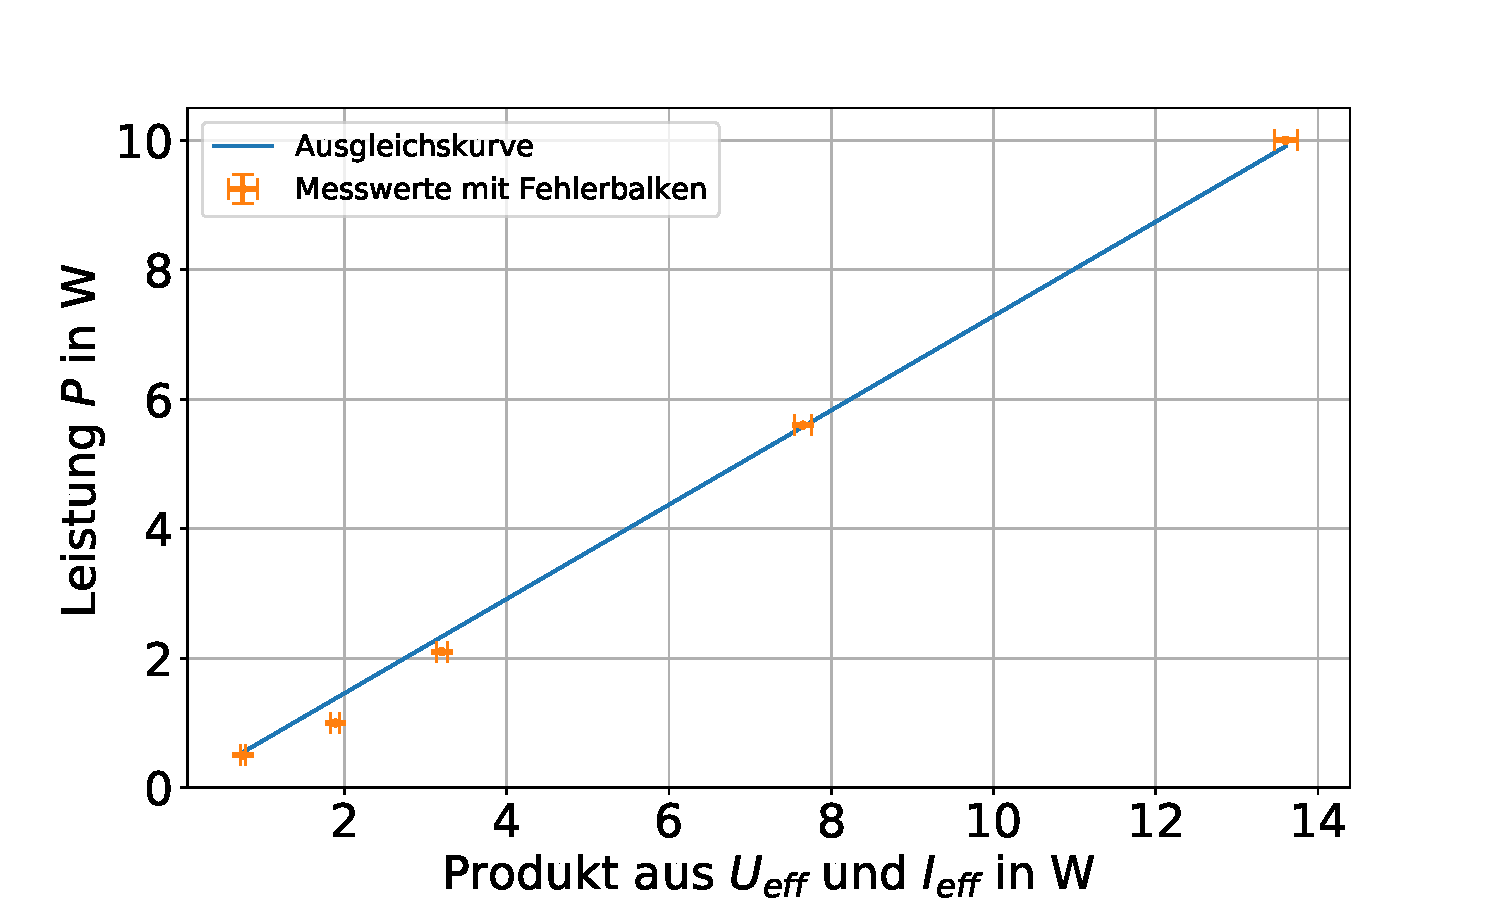
\includegraphics[width=0.9\linewidth]{res/PgegenUI.pdf}
	\caption{Die Leistung P$_\text{eff.}$ gegen $U_{eff.} \cdot I_{eff.}$ für Wechselstrom.}
	\label{fig:PgegenUI}
\end{figure}
Die gemessenen Werte wurden in den Abbildungen \ref{fig:UgegenIgl},  \ref{fig:UgegenIw} und \ref{fig:PgegenUI} dargestellt.
Die für die weitere Auswertung wichtigen Gleichungen lauten:
\begin{align}
	|Z|=\sqrt{R_W + \omega^2L^2}\\
	L=\frac{\sqrt{|Z|^2-R^2}}{\omega}\\
	\label{eq:Indukt}
	|Z|=\frac{U_{eff.}}{I_{eff.}}\\
	\phi = \arccos\left(\frac{\bar{P}}{U_{eff.}I_{eff.}}\right)\\
	R_W=|Z|\cdot \cos(\phi)	\label{eq:R_W}.
\end{align}
(Alle oben genannten Gleichungen gelten für Wechselstrom mit $\omega=2\pi \cdot \SI{50}{Hz}.$)
\begin{align}
	R_i=\frac{U}{I}
\end{align}
(Gilt für Gleichstrom.)\\
Entnimmt man die Steigungen aus den Abbildungen \ref{fig:UgegenIgl}, \ref{fig:UgegenIw} und \ref{fig:PgegenUI} und setzt sie in die oben genannten Gleichungen ein so erhält man die unten zu sehenden Werte. Hierbei wurde jedoch in Gleichung \ref{eq:Indukt} $R_i$ eingesetzt, da $R_i$ direkt aus der Steigung der Abb. \ref{fig:UgegenIgl} abgelesen wurde während $R_W$ durch Gleichung \ref{eq:R_W} berechnet werden musste. Vergleicht man die beiden Werte von $R_w$ und $R_i$ miteinander so erkennt man das  $R_W$ in der $2\sigma$-Umgebung von $R_i$ liegt. 

\begin{align}
		Z &= \SI{29.4+-0.4}{\ohm}\\
		\phi &= \SI{0.7548+-0.0003}{rad}\\
		R_W &= \SI{21.4+-0.3}{\ohm}\\
		R_i &= \SI{22.7+-0.8}{\ohm}\\
		L &= \SI{0,060+-0,004}{H}\\
\end{align}
